\section{tasks::wavecal Class Reference}
\label{classtasks_1_1wavecal}\index{tasks::wavecal@{tasks::wavecal}}
Inheritance diagram for tasks::wavecal::\begin{figure}[H]
\begin{center}
\leavevmode
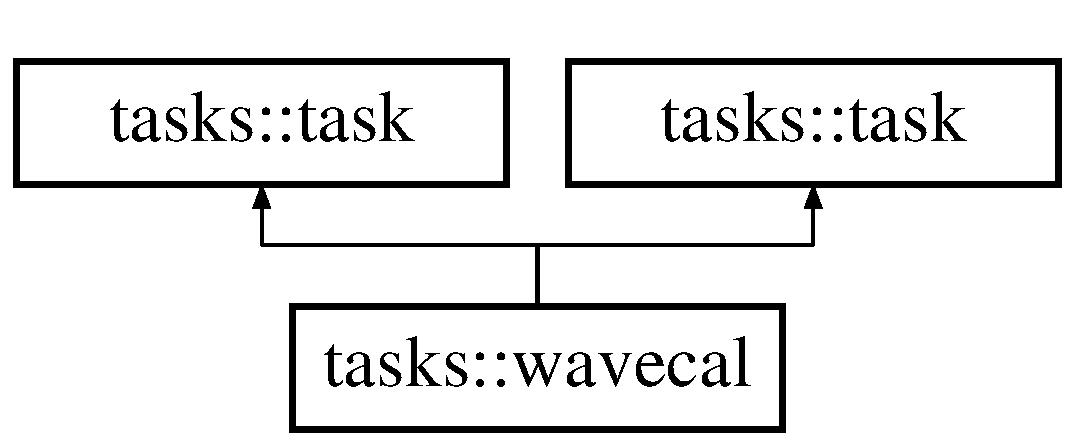
\includegraphics[height=2cm]{classtasks_1_1wavecal}
\end{center}
\end{figure}
\subsection*{Public Member Functions}
\begin{CompactItemize}
\item 
def \textbf{run}\label{classtasks_1_1wavecal_f6be9eb15626e914a716d2cea7dd733a}

\item 
def \textbf{run}\label{classtasks_1_1wavecal_f6be9eb15626e914a716d2cea7dd733a}

\end{CompactItemize}
\subsection*{Static Public Attributes}
\begin{CompactItemize}
\item 
string \textbf{name} = '{\bfwavecal}'\label{classtasks_1_1wavecal_662466b5dca4887cf29a1544ff540e4e}

\item 
string \textbf{button\-Text} = 'Find wavelength solution'\label{classtasks_1_1wavecal_8d305b5a22837dda6b63b083284d3403}

\item 
list \textbf{prereq} = ['{\bffindord}']\label{classtasks_1_1wavecal_00ba057428243ec2132a86836fe0ad1b}

\item 
int \textbf{inthread} = 0\label{classtasks_1_1wavecal_be011617a0ed60b4abde6e02f292027a}

\end{CompactItemize}


\subsection{Detailed Description}


\footnotesize\begin{verbatim}Interactively determine a 2-dimensional wavelength definition from a
   well-exposed wavelength definition frame, normally an ThAr frame.
\end{verbatim}
\normalsize
 



The documentation for this class was generated from the following files:\begin{CompactItemize}
\item 
old/PANICtool-1.0/tasks.py\item 
old/tasks.py\end{CompactItemize}
